\documentclass{ucl_thesis}

%twoside for double page printing
\usepackage{graphics}
\usepackage{graphicx}
\usepackage{color}
\usepackage{verbatim}
\usepackage{algorithm}
\usepackage{algorithmic}
\newcommand{\theHalgorithm}{\arabic{algorithm}}
\usepackage[square]{natbib}

\usepackage[font=footnotesize,labelfont=bf,singlelinecheck=on]{caption}
\usepackage[hyphens]{url}

\usepackage{amsmath}
% Uncomment this to activate the TikZ library, which is useful for fancy block-diagrams.
%    \usepackage{tikz}
%    \usetikzlibrary{positioning,arrows,shapes.misc}
\usepackage{multirow}

%\numberwithin{algorithm}{chapter}
%\usepackage{epsf}
\usepackage{fancyvrb}

%\documentclass[12pt,a4paper]{article}
%\usepackage[utf8]{inputenc}
\usepackage[english]{babel}
%\usepackage{amsmath}
%\usepackage{amsfonts}
%\usepackage{amssymb}
%\usepackage{graphicx}
%usepackage[left=2cm,right=2cm,top=2cm,bottom=2cm]{geometry}
%
%\usepackage[]{natbib}

%% LISTINGS
\usepackage{color}
\usepackage{listings}
\definecolor{mygreen}{rgb}{0,0.6,0}
\definecolor{mygray}{rgb}{0.5,0.5,0.5}
\definecolor{mymauve}{rgb}{0.58,0,0.82}
\definecolor{purple}{rgb}{0.28,0.23,0.5}
\lstdefinestyle{customcpp}{
  belowcaptionskip=1\baselineskip,
  breaklines=true,
  frame=L,
  xleftmargin=\parindent,
  language=C++,
  showstringspaces=false,
  basicstyle=\footnotesize\ttfamily,
  keywordstyle=\bfseries\color{green},
  commentstyle=\itshape\color{purple},
  identifierstyle=\color{blue},
  stringstyle=\color{orange},
  numbers        = left,
  stepnumber     = 5,
}
%%

%% figure template
\newcommand{\myfig}[6]{%
\begin{figure}[h!]\centering%
	\begin{minipage}[b]{0.49\linewidth}\centering%
		\includegraphics[width=\textwidth]{#2}%
		\caption{#3}%
		\label{fig:#1}%
	\end{minipage}%
	\begin{minipage}[b]{0.49\linewidth}\centering%
		\includegraphics[width=\textwidth]{#5}%
		\caption{#6}%
		\label{fig:#4}%
	\end{minipage}%
\end{figure}%
}
%%

%% shortcuts
%Malcolm added some custom commands here - you can make your own!
\newcommand{\vect}[1]{\boldsymbol{#1}}
\newcommand{\figref}[1]{(Fig. \ref{#1})}
\newcommand{\secref}[1]{(Section \ref{#1})}
\def\etal{{et~al.}}
\def\ie{{\it i.e.,\ }}
\def\etc{{\it etc.,\ }}
\def\eg{{\it e.g.,\ }}
\def\vs{{\it vs.\ }}
%%

\author{Aron Monszpart}
\title{Hand-held Scanning of Surface Details}
\def \supervisor {Dr. Gabriel Brostow}
\date{September 2013}

\begin{document}

\bibliographystyle{plainnat}
\maketitle
\numberwithin{algorithm}{chapter}
\setcounter{page}{1}
\pagenumbering{roman}
\pagestyle{plain}

% Notice how the star "*" is used throughout LaTex to modify the normal behavior. For example, \section* instead of \section 
% tells LaTex NOT to number this section.


\newpage
\section*{Abstract}
I've done some stuff
%\input{abstract.tex}


\newpage
\section*{Acknowledgements}
Dr. Gabriel Brostow, Dr Neill Campbell, Dr. Oisin Mac Aodha, Fabrizio Pece, Malcolm Reynolds, Clement Godard, Peter Rennert and the UCL PRISM group

%\setcounter{tocdepth}{2}
\tableofcontents
\listoffigures
%\listoftables
%\listofalgorithms
\newpage

\setcounter{page}{1}
\pagenumbering{arabic}
\pagestyle{plain}

\chapter{Introduction and Background} 

\par The targeted system attempts to solve the problem of 3D reconstruction of fine surface details in static scenes. We have seen various examples of sparse 3D reconstruction methods using the achievements of multi-view stereo, structure from motion and SLAM techniques in \secref{sec:SFM}. In recent years, a large leap has been made in dense 3D reconstruction by methods in \secref{sec:kinfu}. By designing this system we attempted to address inaccurracies produced by the above mentioned methods to refine high frequency details in small segments of the reconstructed models.

\label{chp:background}
	\begin{itemize}	
		\item Motivation
		\item Overview of approach
		\begin{itemize}
			\item Calibration
			\item Low resolution 3D reconstruction
			\item Pose estimation of new input
			\item Mesh subdivision and 2D projection
			\item Depth upsampling
			\item Mesh enhancement by backprojection
		\end{itemize}
	\end{itemize}

\chapter{Related work} 
\label{chp:related_work}

\section{Calibration}
\label{sec:lit_calib}

One of the initial steps of the setup of every multi-camera system has to be calibration. The expression calibration can be interpreted with several meanings. In this document we refer to calibration as the preprocessing step that captures the characteristics of the physical recording system accounting for, amongst others, inaccuracies in the physical manufacturing processes of the cameras. A successful calibration enables a correspondence to be calculated between data captured at the same time with the different cameras. This correspondence is data dependent in the case of depth cameras, and thus calculated every frame.\\

A wider interpretation of calibration includes the calculation of a nearly global position of the recording system. It usually is incorporated by the relative position estimation between the observed scene and the recording system, which can be viewed as global in case the global position of the observed scene is known. \\

Most previous works targeting to develop a highly accurate calibration system agree on the computational parameter model called pinhole-camera model \figref{eq:pinhole}. The model specifies the parameters: focal length ($f_x$, $f_y$), principal point ($c_x$, $c_y$) and skew ($\gamma$).

\begin{figure}[h!]
\begin{equation}
\lambda
\underbrace{
	\left[\begin{array}{ccc}
	    x \\
	    y \\
	    1 \\
	\end{array} \right]
}_{
	{\bf \tilde{x}}_{image}
}
%
=
%
\underbrace{
	\left[\begin{array}{cccc}
			f_x & \gamma & c_x & 0 \\
			0   & f_y    & c_y & 0 \\
	 		0   & 0      & 1   & 0 \\
	\end{array} \right]
}_{
	\left[\begin{array}{cc}
		\bf{\Lambda} & \bf{0}
	\end{array} \right]
}
%
\underbrace{
	\left[\begin{array}{cccc}
	    r_{1,1} & r_{1,2} & r_{1,3} & t_1 \\
	    r_{2,1} & r_{2,2} & r_{2,3} & t_2 \\
	    r_{3,1} & r_{3,2} & r_{3,3} & t_3 \\
	    0       & 0       & 0       & 1 \\
	\end{array} \right]
}_{
	\left[\begin{array}{cc}
		\bf{\Omega}     & \bf{\tau} \\
		\bf{0}^{\it{T}} 	& 1		      \\
	\end{array} \right]
}
%
\underbrace{
	\left[\begin{array}{c}
	    u \\
	    v \\
	    w \\
	    1 \\
	\end{array} \right]
}_{
	{\bf \tilde{x}}_{world}
}
\end{equation}
\caption{Correspondence between a point in global world coordinates (X,Y,Z) and camera image coordinates (u,v) according to the pinhole camera model. Source: UCL 2012 Machine Vision lecture notes. }
\label{eq:pinhole}
\end{figure}

Initial works \citep{Melen:1994}, \citep{Weng:1992} use the combination of linear, and non-linear minimisation techniques to calculate physically based camera parameters. In [9] non-physical implicit parameters are used in a two-step optimisation approach. The baseline calibration technique used in this project relies on the four-step calibration approach presented by \citep{Heikkila:1997}. They introduced a technique to estimate a four component set of distortion parameters in addition to the intrinsics of the pinhole camera. These parameters account for the radial ($k_1$, $k_2$) and tangential ($p_1$, $p_2$) distortion of the camera model. In parallel \citep{Zhang00} published a different camera calibration method only relying on two radial distortion parameters. A widely used implementation of the theoretical achievements of the above works is incorporated in Jean-Yves Bouguet's "Camera Calibration Toolbox for Matlab" \citep{calibration_bouguet}. Here a third order radial distortion parameter $k_3$ is introduced for higher accurracy. The computational model optimised for is described in \figref{eq:distortion}.

\begin{figure}[h!]
    \begin{equation*}
	\left[\begin{array}{c}
		u_{camera} \\
		v_{camera} \\
		w_{camera} \\
	\end{array} \right]
	=
    	\left[\begin{array}{c|c}
	    	{\bf \Omega} & {\bf \tau}
	\end{array} \right]
	\left[\begin{array}{c}
	    u \\
	    	v \\
	    w \\
	\end{array} \right]
    \end{equation*}
    
    \begin{equation*}
	{\bf x}_{normalized} = 
 	\left[\begin{array}{c}
	    \frac{ u_{camera} }{ w_{camera} } \\
	    \frac{ v_{camera} }{ w_{camera} } \\
	\end{array} \right]; 
	~r = length(	{\bf x}_{normalized} )
    \end{equation*}

    \begin{equation*}
	{\bf x}_{undistorted}
	=
	(1 + k_1 r^2 + k_2 r^4 + k_3 r^6 ) {\bf x}_{normalized} 
	~+~ 
	\left[\begin{array}{c}
	    2 p_1 {\bf x}_{normalized,x} {\bf x}_{normalized,y} + p_2 ( r^2 + 2{\bf x}_{normalized,x}^2) \\
	    p_1(r^2+2{\bf x}_{normalized,y}^2) + 2 p_2 {\bf x}_{normalized,x} {\bf x}_{normalized,y}\\
	\end{array} \right]
	\end{equation*}
    \begin{equation*}
		{\bf \tilde{x}}_{image} = {\bf\Lambda} ~ {\bf \tilde{x}}_{undistorted}
    \end{equation*}
    
    \caption{Distortion parameters in the pinhole camera model}
    \label{eq:distortion}
\end{figure}

The achievements of the toolbox were further developed in Intel's \citep{calibration_opencv} package . Additionally, the Graphics and Media Lab of the Lomonosov Moscow State University published a C++ and Matlab calibration toolbox known as \citep{calibration_gml}.
\citep{calibration_rgbdemo}

herrera 13


%http://burrus.name/index.php/Research/KinectCalibration
%vrui
%ros http://wiki.ros.org/kinect\_node/Calibration
%ellipses



\section{Depth upsampling}
\citep{MatsuoFI13} \\
\citep{} TUVienna paper of selfsimilarities

In \citep{Silberman:ECCV12} ... they give a very good kinect dataset for segmentation, use RANSAC and implement cross bilateral filtering

\section{Kinect fusion papers}
\label{sec:kinfu}

%vladlen:
\citep{Zhou:2013}
% mr siggraph 13 kinfu:
\citep{Chen:2013:Scalable_volumetric}
% kintinous 2
\citep{Whelan13iros}
% Kintinuous1
\citep{Whelan12rssw}
% lefloch
Point based Fusion:
\citep{keller13realtime}

Pose estimation improvement: \citep{Whelan13icra}
Multi scale depth: \citep{Fuhrmann:2011}

\section{<planned>}

	\begin{enumerate}
		\item 3D reconstruction using Multi-view stereo
		\begin{itemize}
			\item Curless and Levoy
			\item Rusinkiewicz
			\item Szeliski
			\item Agarwal
			\item Snavely
			\item Seitz
			\item Furukawa and Ponce
			\item Strecha
			\item etc. from literature review (got good marks for it)
			\item Kim et al: Scene reconstruction from High Spatio-Angular Resolution Light Fields (Siggraph '13)
		\end{itemize}

		\item 3D reconstruction using RGB-D
		\begin{itemize}
			\item Voxelgrid based
			\begin{itemize}
				\item Newcombe: Kinect fusion
				\item Whelan: Kintinuous and other loop closure papers
				\item Vladlen: Dense scene reconstruction with points of interest
				\item etc.
			\end{itemize}

			\item Height-field based, layered
			\begin{itemize}
				\item Adaptive voxelgrid based, scene scale aware (Freiburg)
				\item etc.
			\end{itemize}

			\item Point based
			\begin{itemize}
				\item Damien Lefloch
				\item etc.
			\end{itemize}

			
		\end{itemize}
			
 		\item Pose estimation
		\begin{itemize}
			\item some ICP references
			\item Gyro papers
			\item MVS already earlier
		\end{itemize}
		
		\item Upsampling
		\begin{itemize}
			\item RGB superresolution
			\item Depth superresolution
			\begin{itemize}
				\item Non-guided
				\begin{itemize}
					\item Learning based
						\begin{itemize}
							\item Mac Aodha et al. '12
							\item etc.
						\end{itemize}
					\item Other
					\begin{itemize}
						\item Hornacek et al.: Depth Super Resolution by Rigid Body Self-Similarity in 3D, CVPR '13
						\item etc.
					\end{itemize}
				\end{itemize}
				
				\item Guided
				\begin{itemize}
					\item Joint Bilateral
					\begin{itemize}
						\item Yang '07
						\item etc.
					\end{itemize}
					\item MRF based
					\begin{itemize}
						\item Diebel and Thrun
						\item Schuon et al.
						\item Park et al. '11
						\item Choi et al. '12
						\item Shen and Cheung CVPR '13 (Layer Depth Denoising and Completion for Structured-Light RGB-D Cameras)
						\item etc.
					\end{itemize}
					
					\item Spatio-temporal filtering
					
				\end{itemize}
			\end{itemize}
		\end{itemize}
		
		\item Commercial 3D scanners
		\begin{itemize}
			\item MVS based: Photosynth, Adobe, etc.
			\item Laser scanner systems (industrial)
			\item Kinect based: Scanec, Reva, ReconstructMe, ...
		\end{itemize}
		
		\item Seen/used calibration references
		\item Subdivision references
		\item Efficient raycasting references
		\item (+ Categorize all the ref e-mails from Gabriel, Oisin, Reading groups, etc.)
	
	\end{enumerate}

\chapter{MySystem} 
\label{chp:my_system}

\par The targeted system attempts to solve the problem of 3D reconstruction of fine surface details in static scenes. We have seen various examples of sparse 3D reconstruction methods using the achievements of multi-view stereo, structure from motion and SLAM techniques in \secref{sec:SFM}. In recent years, a large leap has been made in dense 3D reconstruction by methods in \secref{sec:kinfu}. By designing this system we attempted to address inaccuracies produced by the above mentioned methods to refine high frequency details in small segments of the reconstructed models. \\

\par The system designed acknowledges the power of SLAM performed on the dense model incorporated in the areas of RGB-D based methods. We also recognize the power of other research areas, where inter-sensory information is used to enhance output quality. We hypothesize that there is information collected by the capturing system but is discarded too early in the reconstruction pipeline of a standard RGB-D system. We looked for methods that enable this information to be reintegrated into the results of the reconstruction at later processing steps. The solution was designed based on the alleged potential of iterative, cost-volume based joint bilateral filtering with sub-pixel accuracy in \citep{cvpr-07-qingxiong-yang}. \\

//TODO: What problem does my system solve?
!any RGB pose refinement!
//TODO: Pipeline image

\section{Assumptions}
\label{sec:assumptions}

\par When designing a system solving a specific problem, it is important to firmly decide what assumptions are made about the input, what problems are targeted to be solved and what problems are out of the scope of the planned method. We target to design a system, that reconstructs fine surface details of static scenes with mostly Lambertian surfaces allowing offline post-processing. \\

\par The fine surface details of a static scene are to be reconstructed. The problems arising when dealing with dynamic scenes are out of scope for this solution. Rigidity is a common assumption in the field of 3D reconstruction both for multi-view stereo and structured lighting methods. An essential building block of our concept is the possibility to later acquire new data about missing details and integrate it into the reconstruction. Since pose estimation of latter acquisitions is a substantial problem on its own, the assumption about static scenes seems reasonable to make. \\

\par Surfaces with close-to Lambertian reflectivity are considered. During experiments refractive and reflective surfaces appeared in the scene, but the main focus of the system development addresses problems emerging around fine details on mostly Lambertian surfaces. \\

\par The solution will perform post-processing offline. The planned key contribution of the work is to acquire surface details at a finer level than current state-of-the art solutions are capable of. As generally in all fields of computer science, a trade-off between quality and speed has to be made. Thus, the planned solutions operate using offline processing and refinement steps. Precedence in similar projects of using offline processing as capabilities of cloud computing has been observed in applications as Adobe Catch \citep{AdobeCatch} or Microsoft Photosynth \citep{Photosynth}. State-of-the art large-scale RGB-D reconstruction algorithms also may operate off-line, as \citep{Zhou:2013}. \\

\section{Calibration}
\label{sec:calibration}

What is calibration, pinhole camera model, different notations (oulu, etc.), 
with IR, without IR
USB bus problems, overlayed image

% Input rgb and depth
\begin{figure}[h!]\centering
    \begin{minipage}[b]{0.49\linewidth}
        \includegraphics[width=\textwidth]{/home/bontius/workspace/cpp_projects/KinfuSuperRes/SuperRes-NI-1-5/build/out/imgs_20130725_1809/img8_00000001.png}
        \caption{Input RGB}
    \end{minipage}
    \begin{minipage}[b]{0.49\linewidth}
        \includegraphics[width=\textwidth]{/media/Storage/Dropbox/UCL/project/results/presentation_300713/dep8_00000001.png}
		\caption{Input depth}
    \end{minipage}
\end{figure}

% Simple alignment
\begin{figure}[h!]\centering
	\begin{minipage}[b]{0.49\linewidth}
		\includegraphics[width=\textwidth]{/media/Storage/Dropbox/UCL/project/results/presentation_300713/dep16AndRgb_00000001.png}
		\caption{No alignment}
	\end{minipage}
	\begin{minipage}[b]{0.49\linewidth}
		\includegraphics[width=\textwidth]{/media/Storage/Dropbox/UCL/project/results/presentation_300713/dep16AndRgb_00000000.png}
		\caption{"Built-in alignment"}
	\end{minipage}
\end{figure}


\begin{figure}[h!]\centering
    \begin{minipage}[b]{0.49\linewidth} \label{fig:ir}
        \includegraphics[width=\textwidth]{/media/Storage/Dropbox/UCL/project/results/presentation_300713/irAndDep8_00000001.png}
        \caption{Default IR and depth overlay}
    \end{minipage}
    \begin{minipage}[b]{0.49\linewidth}
        \includegraphics[width=\textwidth]{/media/Storage/Dropbox/UCL/project/results/presentation_300713/offsIrAndDep8_00000001.png}
        \caption{IR offset by radius of convolution kernel}
    \end{minipage}
\end{figure}

\begin{figure}[h!]\centering
        \includegraphics[width=\linewidth]{/home/bontius/workspace/cpp_projects/KinfuSuperRes/SuperRes-NI-1-5/build/out/imgs_20130725_1809/img8_00000001_mapped.png}
        \caption{Mapping from 640x480 depth to 1280x1024 RGB after calibration}
\end{figure}


default image, built in alignment image, good image\\
calibration papers, and their comparison of optimisation techniques\\
calibration with different sources (depth and acryl, ir, ellipses)\\
cuda mapping\\


\subsection{takeaway}
Ir image with and without projector\\
large checkerboard vs. small checkerboard\\
all positions (mosaic image?)\\
checkerboard sze 
All the squares must be clearly visible (unoccluded).
Use a tripod
Take 25 images and more
Use a paper size ".3" and more
Square size is 3-5 cm
The chessboard on the images must be located in the all places of the camera matrix

\section{3D reconstruction}

The task of accurate real-time mapping of complex and
arbitrary indoor scenes in variable lighting conditions was claimed to have been solved by \citep{Newcombe11}. They list using only a
moving low-cost depth camera and commodity graphics hardware to their contributions as well. There have been made many improvements to the method since it's initial publication detailed in \secref{sec:kinfu}. We base the hypothesis of our work on the claim, that RGB-D reconstruction's attention to the complexity of the scenes can be developed further. Therefore, during the design of the system this algorithm was treated as baseline, its results were reproduced, carefully inspected and an attempt was made to improve upon them. During the extensive research performed to assess the capabilities of derivatives of this algorithm to reconstruct the targeted fine details we did rarely come across projects giving reason to attempt to reproduce their results instead, and treat them as baseline. However, in the future point-based fusion concepts introduced by \citep{keller13realtime} is worth taking into account to improve the starting point of our algorithm.

\myfig
{fig:kinfu_baseline}
{/home/bontius/workspace/cpp_projects/KinfuSuperRes/thesis/img/kinfu_baseline00.png}
{PCL\'s Kinfu output of scene recorded by us}
{fig:lefloch}
{/home/bontius/workspace/cpp_projects/KinfuSuperRes/thesis/img/lefloch_largescale.png}
{\citep{keller13realtime}}

The 
We fuse all of the depth data streamed from a Kinect sensor into
a single global implicit surface model of the observed scene in
real-time. The current sensor pose is simultaneously obtained by
tracking the live depth frame relative to the global model using a
coarse-to-fine iterative closest point (ICP) algorithm, which uses
all of the observed depth data available. We demonstrate the advantages
of tracking against the growing full surface model compared
with frame-to-frame tracking, obtaining tracking and mapping results
in constant time within room sized scenes with limited drift
and high accuracy. We also show both qualitative and quantitative
results relating to various aspects of our tracking and mapping system.
Modelling of natural scenes, in real-time with only commodity
sensor and GPU hardware, promises an exciting step forward
in augmented reality (AR), in particular, it allows dense surfaces to
be reconstructed in real-time, with a level of detail and robustness
beyond any solution yet presented using passive computer vision.

rewrite intro from newcombe

why not sparse, dtam, slam?

\par An easy to operate, hand-held scanning device is used. The developed system will most likely use a smartphone with built in inertial measurement unit, gyroscope, magnetometer and GPS sensor. Alternatively a camera with mounted and calibrated motion and orientation sensors can be used. The performance of structured lighting devices as Microsoft Kinect \cite{Kinect} or Asus Xtion PRO \cite{XtionPro} will also be explored. Eventually a higher resolution device as Leap-motion's gesture recognition solution \cite{LeapMotion} will be evaluated. To ensure interchangeability of the sensors, and to get these systems to cooperate to the highest level possible, a well designed framework needs to be developed. The extensibility of the KinectFusion SDK will be tested once it get's released as part of the Windows 8 SDK as promised \cite{SDKKinectFusion}. Alternatives, as the implementation of a Kinect Fusion like functionality in the Point Cloud Library ("Kinfu") will also be tested \cite{KinFu}.
\par The commercial accessibility of the used sensor setup has a slightly increased emphasis at this stage of the project. Low cost and out of the box operability would open the possibilities for crowd sourcing in follow-up projects, something that has been targeted by many other research labs as Microsoft (at Techfest 2013) or the University of Washington (Photocity, Pointcraft).

PCL steps short description

\section{Yang}

%\lstset{frame=single,language=C++,tabsize=1,basicstyle=\ttfamily\small,}
\lstset{style=customcpp}
\begin{lstlisting}
__device__ float yangRangeDist( float4 a, float4 b, float sigma )
{
    float mod = ( fabs(b.x - a.x) +
                  fabs(b.y - a.y) +
                  fabs(b.z - a.z)  ) / 3.f;
    return __expf(-mod / sigma);
}
template <typename T>
__global__ void
d_cross_bilateral_filterF( T *dOut, int w, int h, size_t outPitch,
                           float range_sigma, int r, bool onlyZeros = false )
{
    int x = blockIdx.x*blockDim.x + threadIdx.x;
    int y = blockIdx.y*blockDim.y + threadIdx.y;

    if (x >= w || y >= h) return;

    float sum = 0.f, factor = 0.f, t = 0.f;
    float4 guideCenter = tex2D( guideTex, x, y );
    T      centerPix   = fetchTexture<T>( x, y );

    // check for early exit
    if ( onlyZeros && (centerPix != 0.f) )
    {
        dOut[y * outPitch + x] = centerPix;
        return;
    }

    // estimate cost volume
    for ( int i = -r; i <= r; ++i )
    {
        for ( int j = -r; j <= r; ++j )
        {
            // read depth
            T curPix = fetchTexture<T>( x+j, y+i );
            // skip, if no data
            if ( onlyZeros && curPix == 0.f )
                continue;
            // read rgb
            float4 guidePix = tex2D( guideTex, x + j, y + i );
            // estimate weights
            factor = cGaussian[i + r] * cGaussian[j + r] *
                     yangRangeDist( guidePix, guideCenter, range_sigma );
            // accumulate
            t   += factor * curPix;
            sum += factor;
        }
    }
    if ( sum > 0.f )
        dOut[y * outPitch + x] = t / sum;
    else
        dOut[y * outPitch + x] = centerPix;
}

\end{lstlisting}

\section{Combined pipeline}
My combined pipleine ( this is what I did, to get the data fro mhere to there. Draw attention to GPU implementations (get credit for it) )

Depth, and RGB
[move depth to RGB space]
[cross filter to fill holes]
kinfu
acquire new rgb
estimate pose
render kinfu model from pose
upsample

\section{Implementation details}
\subsection{Drivers}
\subsection{Third-party libraries}
simultaneous rgb and IR problems
NVIDIA bilateralfiltering sample
PCL
 pcl bilateral upsampling
 \citep{DCBGridStereo}

%%% CHAPTER 5 %%%
\chapter{Validation / experiments}
\label{chp:validation}

%%% SECTION %%%
\section{Structure from motion} 
\label{sec:sfm}

% acerlit image
\myfig
{acerlit_1}
{/home/bontius/workspace/cpp_projects/KinfuSuperRes/thesis/img/acer_lit00706.jpg}
{A frame of video of backside of a monitor}
{acerlit_mesh}
{/home/bontius/workspace/cpp_projects/KinfuSuperRes/thesis/img/acer_lit01.png}
{Visual SFM 3D reconstruction of monitor} 

% oil bottle image
\begin{figure}[h!]\centering
	\begin{minipage}[b]{0.49\linewidth}\centering
		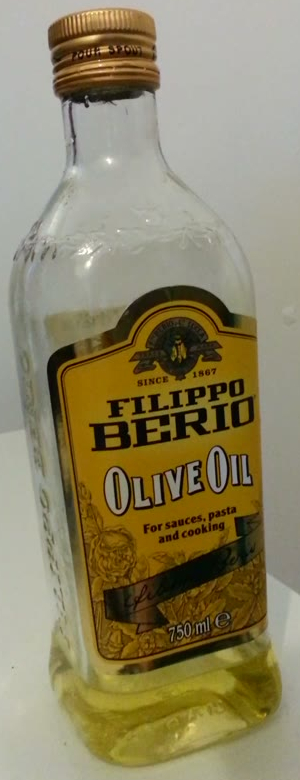
\includegraphics[height=5cm]{/home/bontius/workspace/cpp_projects/KinfuSuperRes/thesis/img/ob00003r2.jpg}
		\caption{A frame of video of oil bottle}
		\label{fig:ob_1}
	\end{minipage}
	\begin{minipage}[b]{0.49\linewidth}\centering
		
\includegraphics[height=5cm]{/home/bontius/workspace/cpp_projects/KinfuSuperRes/thesis/img/ob_mesh00.png}
		\caption{Visual SFM 3D reconstruction of oil bottle}
		\label{fig:ob_mesh}
	\end{minipage}
\end{figure}

%%% SECTION %%%
\section{Iterative joint bilateral upsampling with sub-pixel accuracy}
\label{sec:yang}

\begin{figure}[h!]\centering 
        \includegraphics[width=\linewidth]{/media/Storage/Dropbox/UCL/project/results/final/yang_checkerboard/yanged_nonflat.png}        
        \caption{Example run of implementation on checkerboard scene, results without and with texture after 50 iterations.}
        \label{fig:yang_checkerboard}
\end{figure}

In \figref{fig:yang_checkerboard}

Yang reproductions

Yang does not introduce new depths

%%% SECTION %%%
\section{Results}
\label{sec:results}

\begin{figure}[h!]\centering
    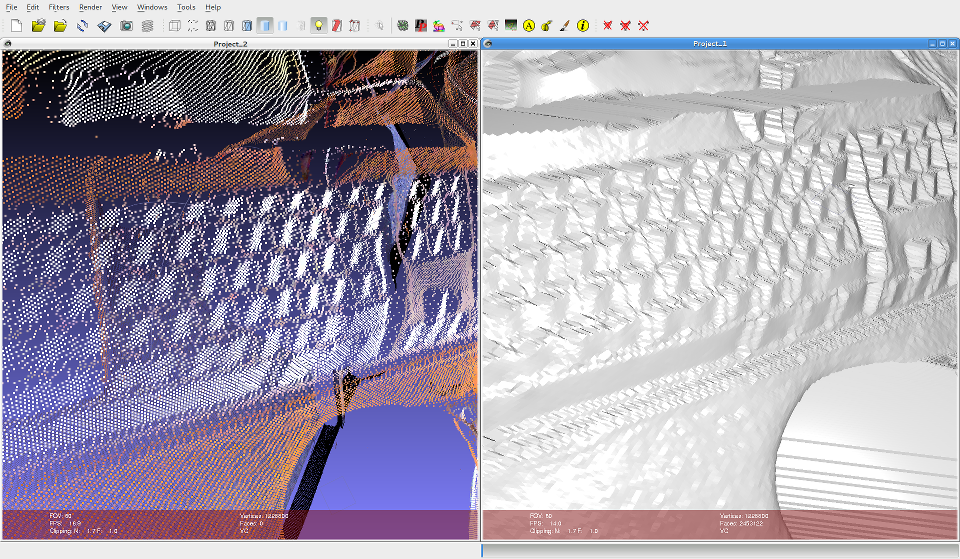
\includegraphics[width=\linewidth]{/home/bontius/workspace/cpp_projects/KinfuSuperRes/thesis/img/keyboard_192_final.png}
    \caption{Close up rendering of keyboard upsampled from skew view angle}
    \label{fig:keyboard_192}
\end{figure}

\begin{figure}[h!]\centering
    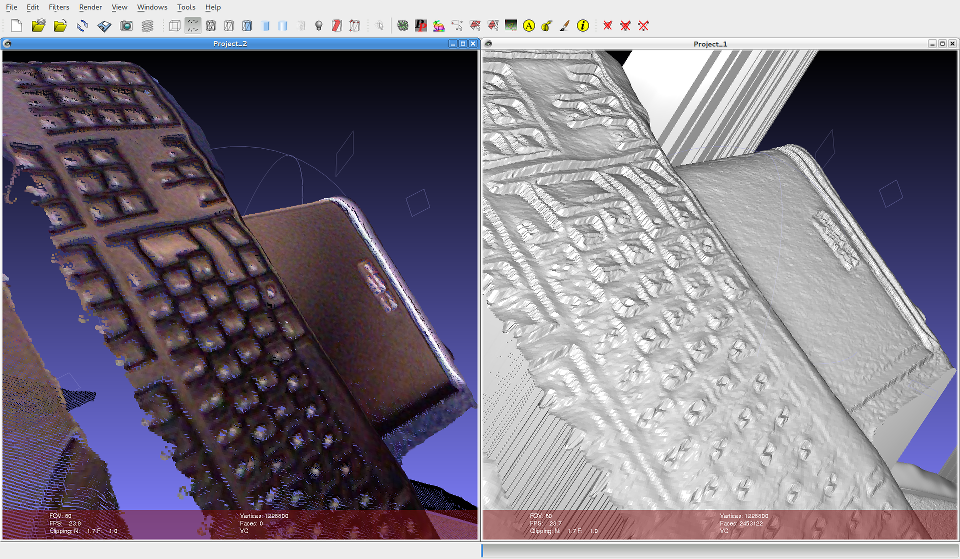
\includegraphics[width=\linewidth]{/home/bontius/workspace/cpp_projects/KinfuSuperRes/thesis/img/keyboard2_192_final.png}
    \caption{Close up rendering of different keyboard upsampled from closer to normal view angle}
    \label{fig:keyboard2_192}
\end{figure}

See meshes on CD

\chapter{Discussion} 
\label{chp:discussion}
    - come back to 3's experiments\\
    - interpret experiments\\
    - did you notice, that 2 were good, and 3rd was abd, remember what I sadi in 3.2, that kinfu does it's calibration...well ,that's crap here (threshold), it happend to be good for 2 sequences, but not their thirds \\
-     Pros, cons \\
- PFM format \\

\section{Limitations} 
\label{sec:limitations}
	- so if Kinfu is not reliable, say it! so if it does not work (pose) than \citep{Whelan13icra} \\
	- misalignment, few frames later, it's great \\
	- calibration \\
    - obvious (Yang on chessboard, it still does) \\
    - summarizing what I discovered \\
    - Kinect RGB quality \\
    - TODO: aligned kinect-rgb, but misaligned kinfu frame example
    
\section{Future work}
- Using segmentation \citep{Silberman:ECCV12} \\
- Occlusion \citep{Hoiem:2011} \\
- Learning based alignment and depth \citep{Herrera:LearnedJointMRF} \\
- put back into mesh (loookup papers!)

This concept fits well into the idea of using a smartphone as sensor in terms of storage space even when recordings of movement sensors' measurements are made. It also fits the concept of an eventual crowd sourcing follow-up project. 

future work: I advocate Yang for the following reasons, or I discourage, since...or in some situations this, than that \\
Kinect \\
Yang \\
Grid recordings of monitor\\


%\section{System plan}
%	\begin{itemize}
%		\item Calibration
%			\begin{itemize}
%				\item Depth image based
%				\item IR image based
%				\item Undistort
%			\end{itemize}
%		\item Low resolution 3D reconstruction
%			\begin{itemize}
%				\item Multi View Stereo (VSFM, Bundler, Photosynth, etc.)
%				\item Kinect Fusion, PCL::Kinfu
%			\end{itemize}
%		\item Pose estimation of new input
%			\begin{itemize}
%				\item VSFM ( for RGB input )
%				\item ICP ( for RGB-D input )
%				\item Gyro+IMU (a noisy graph of acquired data)
%			\end{itemize}
%		\item Mesh subdivision (Linear, Butterfly, Catmull-Clark)
%		\item 2D projection
%			\begin{itemize}
% 				\item Raycasting using Octree
%				\item GLSL projection
%			\end{itemize}
%		\item Yang filtering
%			\begin{itemize}
%				\item Iterative Cross Bilateral filtering
%				\item Subpixel accurracy
%			\end{itemize}
%		\item Mesh enhancement by backprojection
%	\end{itemize}
%	
%\section{System design}
%	\begin{itemize}
%		\item Implementation details and takeaway experience of "System plan" elements
%		\item Merge into previous?
%	\end{itemize}
%	
%\section{Evaluation}
%	\begin{itemize}
% 	\item Experiments
%		\begin{itemize}
%			\item Calibration
%				\begin{itemize}
%					\item Kinect built in calibration
%					\item Bogouet calibration with and without lens distortion (PARAMETERS explained)
%					\item Undistort effectivity (project undistorted depth map to 3D)
%				\end{itemize}
%				
%			\item Filtering
%				\begin{itemize}
%					\item CrossBilateral filter vs. Bilateral
%					\item Yang vs. CrossBilateral (PARAMETERS explained)
%					\item Trilateral, Guided, Pixel Weighted Average Strategy (Garcia et al,ImProc, 2010) - {\bf IF there's time}
%				\end{itemize}
%			\item Kinect fusion related
%			\begin{itemize}
%				\item Kinfu vs. Kinfu w/ filtering turned OFF
%				\item Kinfu voxel grid resolution ($386^3$,$512^3$,$640^3$)
%				\item Kinfu + Yang( original kinect depth frames )
%				\item Kinfu + Yang( "arbitrary pose" )
%			\end{itemize}
%		\end{itemize}
%	\item Existing libraries used
%	\item Data capturing details
%	\item No existing datasets compared (no time)
%
%	\end{itemize}
%
%\section{Results}
%\begin{itemize}
%	\item Upsampling with original depth frames
%	\item Upsampling with simulated "arbitrary pose"
%
%	\item original yang images
%	\item subpixel refinement
%	
%	\item So, Yang is is not suitable for this resolution, it only could improve, when the input was much noisier
%	\item Different approaches can be plugged in to this framework to enhance depth
%\end{itemize}
%\section{Conclusions, Future work}
%	\begin{itemize}
%		\item 3D reconstruction improvements
%			\begin{itemize}
%				\item Improve on smoothing effect of voxel grid weights
%				\item Pose estimation improvements
%			\end{itemize}
%		\item RGB high-resolution capture, vsfm pose estimation 
%		\item Enhancement by best pose selection from input image collection for given pixel/region
%	\end{itemize}
 

\citep{Lowe04}

%\bibliographystyle{plainnat}
\bibliography{litrev}
	
\end{document}


